
\section{The Phase-1 Level-1 Trigger}
\label{section:phase-1-l1-trigger}
% https://cds.cern.ch/record/1556311/files/CMS-TDR-012.pdf
The design performance of the LHC corresponds to an instantaneous luminosity of $10^{34}$ cm$^{-2}$ s$^{-1}$ with a 25 ns bunch crossing rate, giving an average pile-up (number of simultaneous events) of 25 per bunch crossing. The large number of minimum bias events per bunch crossing, combined with the small cross-sections of possible physics discovery signatures, necessitates a sophisticated event selection system for filtering this large event rate, as it is impossible to save all events. This data filtering system is implemented by CMS in two stages. The first stage is the Level-1 (L1) Trigger, which is deployed in custom electronic hardware systems and is responsible for reducing the event rate to around 100 kHz. The second stage is the High-Level Trigger (HLT) which is described in Section \ref{section:phase-1-high-level-trigger}. This section describes the Phase-1 configuration of the Level-1 Trigger.

% CITE: https://cds.cern.ch/record/1556311/files/CMS-TDR-012.pdf
\begin{figure}[ht]
    \centering
    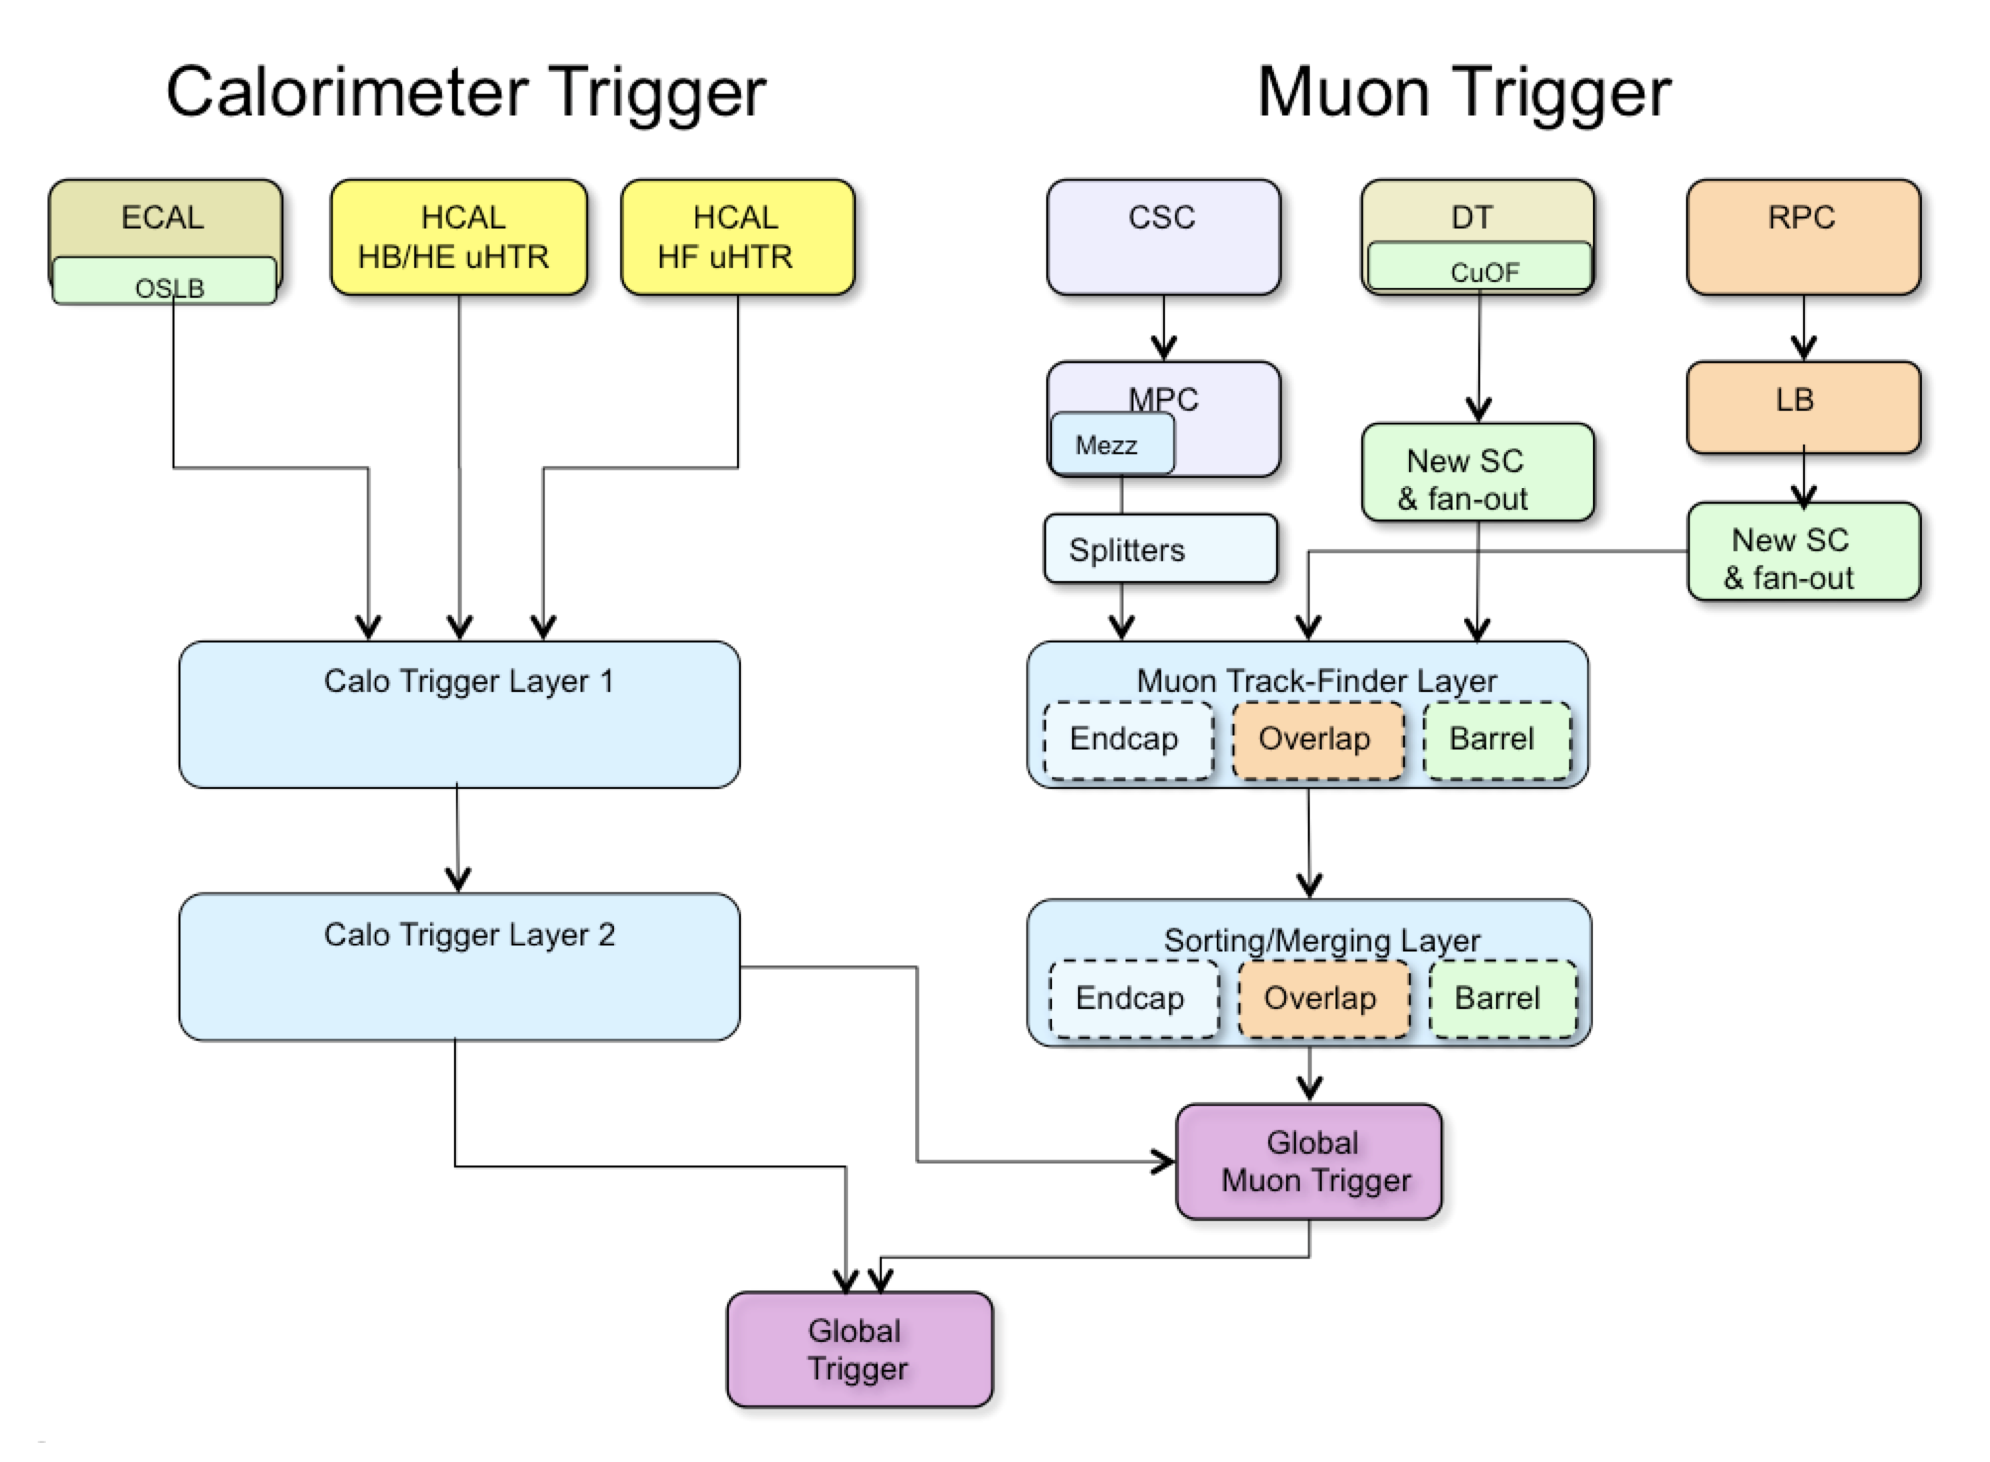
\includegraphics[width=11cm]{figures/ch-3-phase1-l1-trigger/phase-1-level-1-trigger-dataflow.png}
    \caption{Dataflow for the Phase-1 Level-1 Trigger [CITE], which is implemented in custom hardware and is responsible for reducing the event rate from the LHC bunch crossing frequency of 400 MHz (bunch crossings every 25 ns) to a maximum rate of 100 kHz. In Phase-1, the Level-1 Trigger has access to information from the calorimeter and muon detectors.}
    \label{fig:phase-1-level-1-trigger-dataflow}
\end{figure}


% CITE: https://cds.cern.ch/record/1556311/files/CMS-TDR-012.pdf
The L1 Trigger data flow of Phase-1 is shown in Fig. \ref{fig:phase-1-level-1-trigger-dataflow}, with organization into the L1 calorimeter trigger, the L1 muon trigger, and the L1 global trigger. 

% CITE: original trigger configuration: https://cds.cern.ch/record/706847/files/cer-002248791_LHCC-2000-38.pdf
The L1 calorimeter trigger begins with trigger tower energy sums formed by the ECAL, HCAL, and HF Trigger Primitive Generator (TPG) circuits from the individual calorimeter cell energies. In the original configuration, the ECAL energies were accompanied by a bit indicating the transverse extent of the electromagnetic energy deposits, and the HCAL energies were accompanied by a bit indicating the presence of minimum ionizing energy [CITE]. Between Long Shutdowns 1 and 2 (LS1 and LS2), HF was upgraded to provide finer granularity information to the trigger, and the HCAL barrel and endcap front-end electronics were upgraded to provide high-precision timing information and depth segmentation information. 

% CITE https://cds.cern.ch/record/1556311/files/CMS-TDR-012.pdf
In the original design of the L1 calorimeter trigger, the trigger primitives are processed by the Regional Calorimeter Trigger (RCT, upgraded to Calo Layer 1 after LS2) which finds isolated and non-isolated electron/photon candidates. (At this stage, electrons/photons candidates are treated together since they cannot be definitively distinguished at this stage due to lack of tracking information in the L1 trigger.) The Global Calorimeter Trigger (GCT, upgraded to Calo Layer 2 after LS2) sorts further the candidate electrons/photons, finds jets (classified as central, forward, and tau) using the $E_T$ sums and performs calibration of the clustered jet energies, and calculates global quantities such as missing $E_T$. It sends the top four candidates of each type to the global trigger (GT).

% CITE: original trigger configuration: https://cds.cern.ch/record/706847/files/cer-002248791_LHCC-2000-38.pdf
Each of the L1 muon triggers has its own trigger logic. The RPC strips are connected to a Pattern Comparator Trigger (PACT), which forms trigger segments that are used to build tracks and calculate $p_{T}$. The RPC logic also provides some hit data to the CSC trigger system to resolve ambiguities caused by two muons in the same CSC. The CSCs form local charged tracks (LCTs) from the cathode strips, which are combined with the anode wire information. LCTs are combined into full muon tracks and assigned $p_{T}$ values. 

% CITE: original trigger configuration: https://cds.cern.ch/record/706847/files/cer-002248791_LHCC-2000-38.pdf
The Global Muon Trigger (GMT) sorts the RPC, DT, and CSC muon tracks, converts these tracks to the same $\eta$, $\phi$, and $p_{T}$ scale, and validates the muon sign. It improves the trigger efficiency by merging muon candidates that were detected in two complementary sub-systems (i.e. DT+RPC, or CSC+RPC). The GMT also contains logic to correlate the found muon tracks with an $\eta-\phi$ grid of quiet calorimeter towers to determine if the muons are isolated, as well as logic to remove duplicate candidates originating in the overlap regions from both DT and CSC systems. The final collection of muons are sorted based on their initial quality, correlation, and $p_{T}$, and the top four muons are sent to the Global Trigger. 

Information from the GCT and GT are sent to the Global Trigger (GT), which makes the Level-1 Accept (L1A) decision to either discard or accept the bunch crossing. This is accomplished by sorting ranked trigger objects that are accompanied by positional information in $\eta$ and $\phi$, permitting the trigger to applying criteria with thresholds that can vary based on the location of the trigger objects, and/or to require trigger objects to be close to or opposite from each other. The GT L1A decision arrives at the detector front end with a 3.8 $\mu$s latency after the interaction at a rate which is required to be less than 100 kHz, and triggers a full readout of the detector for further processing.

